\chapter{Vorlesungen}
%
%
%
\section{Java-Editionen}
	\begin{itemize}
	\item Java läuft auf sehr unterschiedlichen Systemen
	\item  Wird in verschiedenen „Packungsgrößen“ angeboten
	\begin{itemize}
		\item EE (enterprise edition): große Unternehmensserver
		\item SE (standard edition): Desktop-Systeme
		\item ME (micro edition): Handys, PDAs, Embedded Systems
	\end{itemize}
	\item Editionen unterscheiden sich in den mitgelieferten Zugaben,nicht in der Programmiersprache
	\end{itemize}
%
%
%
\section{Java-Entwicklungssystem}
\begin{itemize}
\item Zum Schreiben neuer Programm ist der Compiler javac nötig, zum Ausführen fertiger Programm nicht
\item  Java für verschiedene Einsatzzwecke:
	\begin {itemize}
		\item JRE (java runtime environment): zum Ausführen fertiger Programme
		\item JDK (java development kit): JRE + Compiler und weitere Hilfsmittel zum Schreiben neuer Programme
	\end{itemize}
\end{itemize}
 %
 %
 %
 \section{Namen in Java}
 \begin{itemize}
 \item An vielen Stellen frei wählbare Namen = „Bezeichner“, „Identifier“
 \item Bestandteile: Große und kleine Buchstaben, Ziffern, Underscore (\_)
 \item Erstes Zeichen darf keine Ziffer sein
 \item Etwa fünfzig reservierte Wörter dürfen nicht als Identifier benutzt werden (beispielsweise class, int, public)
	 \item Beispiele:
 	\begin{itemize}
		\item Counter
		\item colorDepth
		\item Iso9660
		\item XMLProcessor
		\item MAX\_VALUE
	\end{itemize}
	\item Nicht erlaubt sind z.B.:
	\begin{itemize}
		\item1stTry 	(erster Buchstabe darf keine Ziffer sein)
		\item Herz Dame (Leerzeichen im Namen nicht erlaubt)
		\item const (reserviertes Wort)
		\item muenchen-erding (Bindestrich im Namen nicht erlaubt)
	\end{itemize}
	\item Übliche Konventionen für Java-Identifier:
	\begin{itemize}
		\item Variablen, Methoden, primitive Typen: CamelCode, erster Buchstabe klein: counter, find1stToken, bottomUp
 		\item Referenztypen: CamelCode, erster Buchstabe groß: Hello, String, ServerSocket
		\item Typvariablen (Generics): einzelne große Buchstaben: T, U
		\item statische, öffentliche Konstanten: alle Buchstaben groß, Wortteile getrennt mit Underscore: MAX\_VALUE, PI, RGB24
	\end{itemize}
\end{itemize}
%
%
%
\section{Regel Ebenen}
\subsection{Syntax (Rechtschreibung)}
Verteilung von Semikolons, Klammern, Schreibweise von Namen
\subsubsection{Syntaxfehler}
Compiler meldet einen Fehler

\subsection{Semantik (Bedeutung)}
Zulässige Kombination von Sprachelementen
\subsubsection{Semantikfehler}
Compiler meldet einen Fehler, Programm verhält sich falsch, stürzt
nach dem Start ab, ...

\subsection{Pragmatik (Gebrauch)}
Bewährte und sinnvolle Konstruktionen
\subsubsection{Fehler der Pragmatik}
Programm ist unleserlich, umständlich, unverständlich
%
%
%
\section{Polymorphismus}
\begin{itemize}
	\item Der Typ des Ergebnisses, und u.U. der Wert, ist abhängig von
	den Typen der Operanden:
	\begin{description}
		\item []$ 20/8 \rightarrow 2 $
		\item []$20.0/8.0 \rightarrow 2.5$
	\end{description}
	\item Zwei Operanden gleichen Typs: Operandentyp = Ergebnistyp
	\item Gemischte Operandentypen: double-Ergebnis:
	\begin{description}
		\item [] $1 + 2 \rightarrow 3$ (int)
		\item [] $1.0 + 2 \rightarrow 3.0$ (double)
		\item[] $1 + 2.0 \rightarrow 3.0$ (double)
		\item[] $1.0+2.0 \rightarrow 3.0$ (double)
	\end{description}
\end{itemize}
%
%
%
\section{Explizite Typkonversionen}
\begin{itemize}
	\item Hohe Priorität, wie andere unäre Operatoren:
	\begin{description}
		\item [] (int)$2.5*3\rightarrow 2*3 \rightarrow 6$
		\item [] -(int)$2.5 \rightarrow -2$
		\item [] Klammern hilft: (int)$(2.5*3) \rightarrow (\textrm{int})(7.5) \rightarrow 7$
	\end{description}
	\item ACHTUNG STOLPERFALLE
	\begin{description}
		\item[] (int)$1e100 \rightarrow 2147483647$
	\end{description}
	\item Typcasts auf ein Minimum beschränken.
\end{itemize}
%
%
%
\section{Struktogramme}
\begin{itemize}
	\item Elementarbausteine von Struktogrammen: einfache Anweisungen
	\item Formulierung einzelner Anweisungen
	\item Beschreibungs- oder Darstellungsformen für Algorithmen:
	\begin{itemize}
		\item Umgangssprache \\
		Problematisch: Mißverständnisse, Interpretationsmöglichkeiten, 
		Sprachkenntnisse
		\item Quelltext\\
		Nur mit Kennnis einer konkreten Programmiersprache lesbar
		\item Neutrale, abstrakte Form\\
		Brauchbarer Kompromiss
	\end{itemize}
	\item Populär: Struktogramme (=Nassi-Schneiderman-Diagramme)
	\item Früher auch: Flussdiagramme (flow charts), erlauben wirre Konstruktionen
	\item Ziel: Reduktion auf die Idee, die wesentlichen Strukturen
\end{itemize}
\subsection{Umgangssprachlich}
Definiere n als ganze Zahl\\
Gib n den Wert 4\\
Zähle n um 1 hoch\\
Gib n aus\\
\subsection{Pseudocode}
int n\\
n = 4\\
n = n + 1\\
print n\\
\subsection{Nassi-Schneiderman}
\begin{figure} [H]
	\centering 
	\scalebox{0.6}{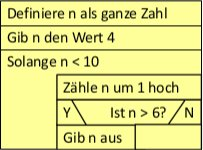
\includegraphics{mainmatter/pics/strukto.jpg}}
	\caption{ein mini Struktogramm} 
\end{figure}
%
%
%
\section{While-Schleife: Euklidischer Algorithmus}
 \begin{lstlisting}[language=JAVA]
class EuclidGCD
{
	public static void main(String... args)
	{
		int m = Integer.parseInt(args[0]);
		int n = Integer.parseInt(args[1]);
		int r = m % n;
		while (r != 0)
		{
			m = n;
			n = r;
			r = m % n;
		}
		System.out.println(n);
	}
}
\end{lstlisting}
%
%
%
\newpage
%
\section{While-Schleife: Collatzfolge (3n + 1 – Folge)}
$z_{n+1} = \left\{ \begin{array}{ll}
         \frac{1}{2}z_{n}, & z_{n}\textrm{ gerade}\\
         3 \cdot z_{n}+1, & z_{n}\textrm{ ungerade}.\end{array} \right. $\\
 \begin{lstlisting}[language=JAVA]
class CollatzMax
{
	public static void main(String... args)	
	{
		int z = Integer.parseInt(args[0]);
		int n = 0;
		int max = z;
		while (z != 1)
		{
			if (z%2 == 0){
				z = z/2;
			}
			else{
				z = 3*z + 1;
			}
			n++;
			if (z > max){
				max = z;
			}
		}
		System.out.println(n);
		System.out.println(max);
	}
}
 \end{lstlisting}
 %
 %
 %
 \section{Inkrement-/Dekrementoperator}
Variable ++; \qquad Variable - -;
 \begin{lstlisting}[language=JAVA]
 int a = 1;
int b = a++; // b = 1, a = 2
int c = a--; // c = 2, a = 1
 \end{lstlisting}
 \qquad\\
++Variable; \qquad - -Variable;
 \begin{lstlisting}[language=JAVA]
int a = 1;
int b = ++a; // b = 2, a = 2
int c = --a; // c = 1, a = 1
 \end{lstlisting}
 %
 %
 %
 \section{Der bedingte Operator}
 \begin{itemize}
 \item Dreistelliger "bedingter Operator" (engl. "conditional operator")
	\item Syntax: \\
		 condition? yes-expression: no-expression
	\item Beziehung zu if:\\
		 variable = condition? yes-expression: no-expression;
	\item äquivalent zu:\\
		 if (condition)\\
		. \qquad variable = yes-expression;\\
		 else\\
		. \qquad variable = no-expression;\\
\end{itemize}
%
%
%
\section{do-while}

\begin{figure} [H]
	\centering 
	\scalebox{0.3}{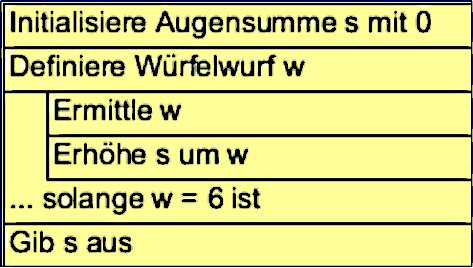
\includegraphics{mainmatter/pics/dowhile.jpg}}
	\caption{ein mini Struktogramm} 
\end{figure}

 \begin{lstlisting}[language=JAVA]
int s = 0;
int w;
do{
	w = // wuerfeln ...
	s += w;
} while (w == 6);
System.out.println(s);
 \end{lstlisting}
%
%
%
\section{Break und Continue}

\subsection{Break}
\begin{itemize}
\item Anweisung break beendet eine Schleife sofort der Rest des Rumpfes wird übersprungen
\item break = einfache Anweisung (wie Definitionen, Wertzuweisungen)
\item Zweck: Entscheidung über Fortsetzung einer Schleife fällt mitten im Rumpf
\end{itemize}

\subsection{continue}
\begin{itemize}
\item Anweisung continue startet sofort den nächsten Schleifendurchlauf der Rest des Rumpfes wird übersprungen
\item Wie break: Nützlich zur Behandlung von Sonderfällen
\item Zweck: Folge von Entscheidungen über Fortsetzung des Schleifendurchlaufes mitten im Rumpf
\end{itemize}	
Achtung: break und continue spalten Kontrollfluss: mit Bedacht
verwenden
%
%
%
\section{Gültigkeitsbereiche}
\begin{itemize}
	\item Idee
	\begin{itemize}
		\item Blöcke {...} gruppieren Anweisungen
		\item Innnerhalb eines Blocks alle Anweisungsarten erlaubt, auch Definitionen
		\item Gültigkeitsbereich (engl. „scope“) einer Variablen...
		\begin{itemize}
			\item beginnt mit der Definition und
			\item endet mit dem Block, in dem die Definition steht
		\end{itemize}
		\item Außerhalb des Blocks: Variable gilt nicht
		\item Gültigkeitsbereiche bezogen auf Quelltext, werden vom Compiler 			
			überprüft
		\item Zur Laufzeit irrelevant
	\end{itemize}
	\item Namenskollision
	\begin{itemize}
		\item Gültigkeitsbereich umfasst untergeordnete (geschachtelte) Blöcke
		\item Namenskollision: Definition des gleichen Namens, wie in einem 	
			umfassenden Block
		\item Java: Doppelte Definition unzulässig
		\item Aber: Kein Problem in disjunkten Blöcken:
	\end{itemize}
\end{itemize}
%
%
%
\section{for-Schleife}
Jede For-Schleife kann durch eine While Schleife ersetzt werden. 
 \begin{lstlisting}[language=JAVA]
for(int i = 0; i < 10; i++)
	System.out.println(i);
 \end{lstlisting}
 %
 %
 %
 \section{Switch}
 \begin{itemize}
 \item Der Wert der expression wird einmal berechnet.
\item Das Ergebnis wird nacheinander mit den labels verglichen, bis zum ersten gleichen Wert.
\item  Die dem label nachfolgenden statements werden ausgeführt, bis zum break;
\item Ziel: switch-Anweisungen ersetzen längere, unübersichtliche if-Kaskaden
\item  Syntax:
\end{itemize}
 \begin{lstlisting}[language=JAVA]
switch (expression)
{
	case label1:
		statement ...
		break;
	case label2:
		statement ...
		break;
	...
}
 \end{lstlisting}
